\section{MoEBIUS: Mixture of Experts and BIclustering Unified Strategy}




\subsection{Model}
MoEBIUS relies on incorporating a conditional variable stratification mechanism within Mixtures of Experts. To achieve this, we introduce a new random variable, denoted as $\bW$.
The purpose of the variable $\bW$ is to determine which covariables are considered and how they are utilized for prediction. This leads us to the following general formulation:
%
\begin{equation}
    \p\left(\by, \bW, \bZ \mid \bX, \bbeta, \brho, \bpi\right) = \underbrace{\p\left(\by \mid  \bW, \bZ,\bX, \bbeta\right)}_{\text{Experts}} 
    \underbrace{\p\left( \bW \mid \bZ, \bX, \brho\right) }_{\text{Variable stratification}} 
    \underbrace{\p\left( \bZ \mid \bX,\bpi\right)}_{\text{Gating network}}.
\end{equation}
At this stage, the specific dimensions of variables are not crucial; these details will be provided in Section \ref{sec: MoEBIUS_Model}.

The definition of experts and the law associated with \( \by \) are intrinsically dependent on the nature of the data. However, they can be formalized through a function \( f \) such that \( f(\by, \bW, \bZ, \bX, \bbeta) \), with $\bbeta$  the expert parameters.
The variable \( \bW \) is influenced by both \( \bZ \) and \( \bX \), allowing for a stratification that depends simultaneously on the communities and the individual-specific characteristics. Finally, the modeling of communities via \( \bZ \) is itself conditioned by \( \bX \); however, a marginal law could be considered.

\subsection{Mixture Of Experts and BIclustering Unified Strategy model}
\label{sec: MoEBIUS_Model}
As in \cite{courbariaux2022sparse}, the assignment to a community is obtained through a multiclass regression.
\begin{equation}
\label{eq: moebius_Z_eq}
    \bZ_{i} \mid \bX_i \sim \M\left(1; \softmax\left(\bX_i \bpi \right) \right),
\end{equation}
where $\bpi$ is a matrix of dimension $p \times K$. 

The goal is to predict the latent variable \( \bZ_+ \) for a new observation \( \bX_+ \), leveraging information obtained during model training. In this context, a regression-based approach is more appropriate than a marginal distribution, as it directly incorporates the relationships learned between the input variables and the latent variables.

Now, based on the Conditional Latent block Model (CLBM) approach developed by \cite{goffinet2020conditional}, we define the \( K \times p \times Q \) tensor \( \bW \), which models the partition of the \( p \) variables into \( Q \) components. 

These partitions are conditioned by the \( K \) communities, meaning that for each community \( k \), the partition of the variables may differ, hence introducing the conditional aspect.
%
Conditionally to the cluster $k$, each row of the component membership matrix follows: 
%
\begin{equation}
\label{eq: moebius_W_eq}
    \bW_{kj} \sim \M\left(1; \brho_k = \left(\rho_{k1},\dots,\rho_{kQ}\right) \right).
\end{equation}
One could have considered incorporating the contribution of \( \bX_i \) in the modeling process, allowing for a partition dependent on the individual rather than the community. However, this would have complicated the interpretability. The rationale behind this approach is to partially summarize the behavior of individuals through the communities to which they belong, making this modeling choice preferable.

In addition, an analysis of the effectiveness of the CLBM under the assumption of constant communities and conditional variable partitions has been conducted, through a study of the Co-Conditional Latent Block Model (\textit{Co-CoLBM}). Parameter estimation, model selection and performance on simulated data have been studied. The code is available on Github (\url{https://github.com/Kdesantiago}).
The detailed results of this study are presented in Appendix \ref{sec: CocoLBM}.


\begin{figure}[!ht]
     \centering
     \begin{subfigure}[b]{\textwidth}
         \centering
         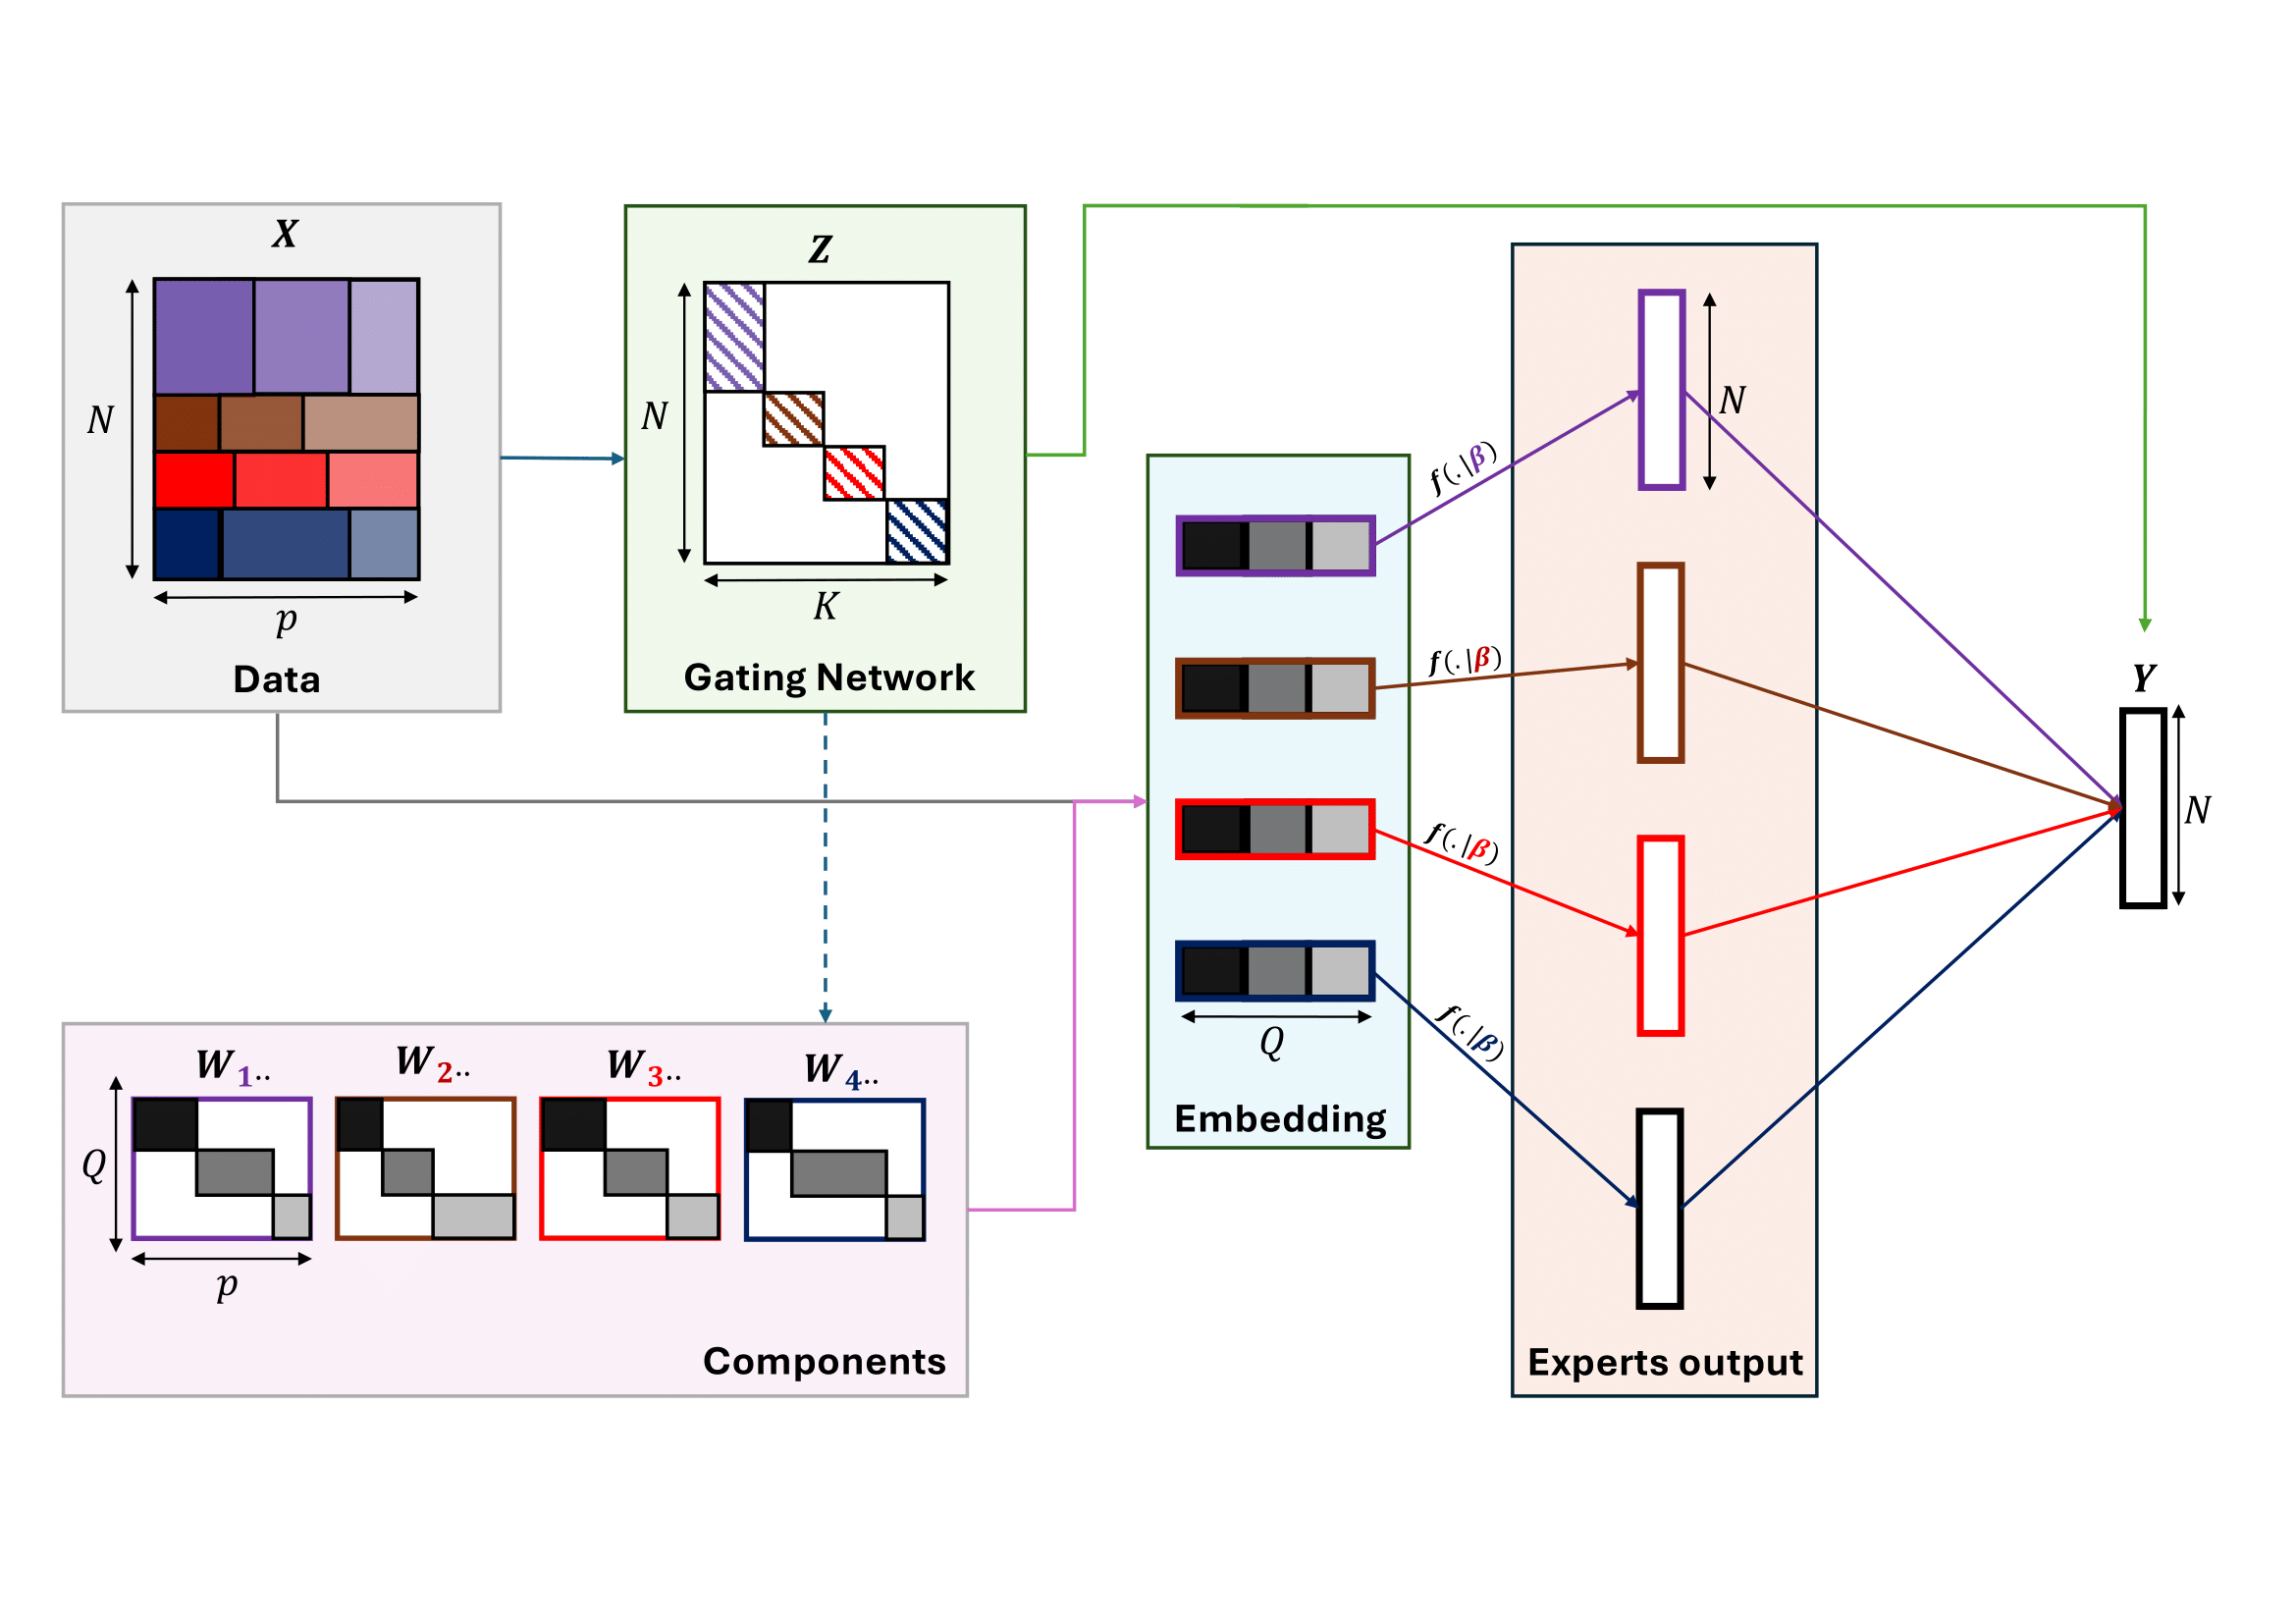
\includegraphics[width=\textwidth]{Figures/CocoLBMoE.png}
     \end{subfigure}
     \hfill
     \caption{ Schematic representation of \textit{MoEBIUS}.
     The input data \( \bX \), of dimension \( N \times p \), is used to define selection weights for the $K$ experts (gating network $\bZ$, with $K$ communities).
     Each expert is associated with a projection matrix \( \bW_k \), of dimension \( p \times Q \), that groups the covariates into components. The data, coupled with the projection matrices, are transformed into matrices of size \( N \times Q \), which are then passed through a regression function \( f_k(. \mid \bbeta_k) \) specific to each expert. 
     The outputs of the experts are combined according to the gating network's weights (based on community membership) to produce a final prediction \( \by \), representing the target variable.}
     \label{fig: CocoLBMoE}
\end{figure}

In modeling the response variable $\by$ conditionally on covariates $\bX$ and latent variables $\bZ$ and $\bW$, different strategies can be employed depending on the nature of the response variable's support.
In this chapter, we focus on two primary settings: regression for continuous outcomes and multinomial logistic regression for categorical outcomes.

\paragraph{Regression} When the support of $\by$ lies in $\mathbb{R}^N$, we adopt the following regression model:
\begin{equation}
y_i \mid \bX_i, Z_{ik} = 1, \bW_{k} \sim \mathcal{N}\left(y_i; \bX_i \bW_{k} \bbeta_k, \sigma^2_k \right) .
\label{eq: reg_CCLBM} 
\end{equation}
In this formulation, the regression parameters $\bbeta_k \in \mathbb{R}^Q$ for each latent class $k$ must be estimated, and $\sigma^2_k$, representing the class-specific noise variance, too.

\paragraph{Multinomial logistic regression} For the case where the support of $\by$ is $\left\{1, \dots, C\right\}^N$, we use a multinomial logistic regression type model:
%
\begin{equation} 
y_i \mid \bX_i, Z_{ik} = 1, \bW_{k} \sim \M\left(1; \softmax\left( \bX_i \bW_{k} \bbeta_k \right)\right).
\label{eq: classif_CCLBM} 
\end{equation}
In this case, the classification parameters $\bbeta_k \in \mathbb{R}^{Q \times C}$ are parameter matrices corresponding to each latent class $k$.

For a given community \( k \), this model can be interpreted as a regression on the vector \( (\bX_i \bW_{k }) \in \mathbb{R}^Q \). The components of this vector represent synthesized features of individual \( i \), conditioned on the partition of community \( k \), and reduced to \( Q \) variables. In other words, the \( p \) original variables are summarized into \( Q \) representative variables, each corresponding to a specific component. The graphical representation of the proposed model is provided in Figure \ref{fig: MoEBIUS Rep Graphique}.
%
\begin{figure}[!ht]
     \centering
     \begin{subfigure}[b]{\textwidth}
         \centering
         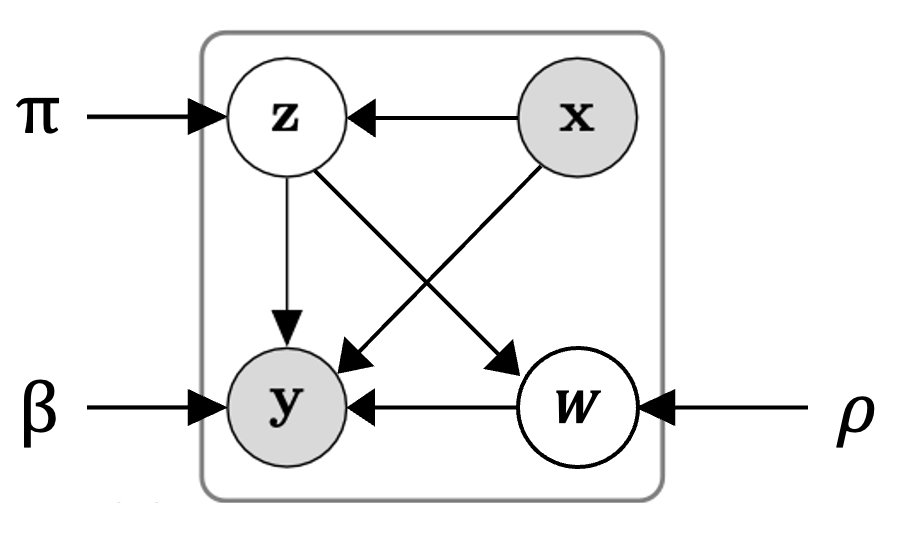
\includegraphics[width=0.6\textwidth]{Figures/CocoLBMoE_repres.png}
     \end{subfigure}
     \hfill
     \caption{Graphical model for \textit{MoEBIUS}. The joint distribution can be factorized as follows:\newline $\p(\by,\bZ,\bW \mid \bX,\bpi, \brho, \bbeta) = \p(\by \mid \bX,\bZ,\bW, \bbeta) \p(\bW \mid \bZ, \brho) \p(\bZ \mid \bX,\bpi)$.}
     \label{fig: MoEBIUS Rep Graphique}
\end{figure}

The complete likelihood can be expressed as:
%
\begin{align}
    \mathcal{L}^c\left(\bbeta, \brho, \bpi; \by,\bZ,\bW \mid \bX\right) &= \p\left(\by,\bZ,\bW \mid \bX, \bpi, \brho, \bbeta   \right) \notag \\
    &= \prod_{i=1}^N \prod_{k=1}^K \p\left(y_i \mid \bZ_{i k},\bW_{k},\bX_i, \bbeta_k   \right)
    \prod_{k=1}^K \prod_{j=1}^p \p\left(\bW_{kj} \mid \bZ,  \brho \right) \notag \\
    &\quad \prod_{i=1}^N  \p\left(\bZ_{i} \mid  \bX_i, \bpi   \right).
\end{align}
% Now, when modeling the target variable $\by$ conditionally on covariates $\bX$ and latent variables $\bZ, \bW$, the problem can be approached in various ways depending on the support of $\by$.

% In this work, we focus on two approaches: regression and multiclass classification.

% \paragraph{Regression}
% Assuming that the support of $\by$ is $\mathbb{R}^N$, we model the target as follows:

% \begin{equation}
%     y_i \mid \bX_i, Z_{ik} = 1 , \bW_{k\bullet\bullet} \sim  \mathcal{N}\left(y_i; \bX_i  \bW_{k\bullet\bullet} \bbeta_k, \sigma^2_k \right)
%     \label{eq: reg_CCLBM}
% \end{equation}

% Here, the regression parameters $(\bbeta_k)_{k=1:K}$ are vectors in $\mathbb{R}^Q$ that need to be estimated.

% \paragraph{Multiclass Classification}
% Assuming that the support of $\by$ is $\left\{1,\dots,C \right\}^N$, we model the target as follows:

% \begin{equation}
%     y_i \mid \bX_i, Z_{ik} = 1 , \bW_{k\bullet\bullet} \sim \M\left(y_i; \softmax\left( \bX_i  \bW_{k\bullet\bullet} \bbeta_k \right) \right)
%     \label{eq: classif_CCLBM}
% \end{equation}

% Here, the classification parameters $(\bbeta_k)_{k=1:K}$ are matrices in $\mathbb{R}^{Q \times C}$ that need to be estimated.



% Thus, the complete likelihood can be written as:

% \begin{align}
%     \mathcal{L}^c\left(\bTheta ; \by,\bZ,\bW \mid \bX\right) &= \p\left(\by,\bZ,\bW \mid \bX, \bTheta   \right) \notag \\
%     &= \prod_{i=1}^N \prod_{k=1}^K \p\left(y_i \mid \bZ_{ik},\bW_{k\bullet \bullet},\bX_i, \bbeta_k   \right)
%     \prod_{k=1}^K \prod_{j=1}^p \p\left(\bW_{kj} \mid \bZ_{ik},  \brho \right) \notag \\
%     &\quad \prod_{i=1}^N  \p\left(\bZ_i \mid  \bX_i, \bpi   \right)
% \end{align}



\subsection{Model Selection}

The model selection process for \textit{MoEBIUS} is based on the ICL criterion proposed by \cite{goffinet2020conditional} for conditional co-clustering and the BIC criterion introduced by \cite{schwarz1978estimating} to penalize the regression component.

\begin{align}
    \operatorname{BIC\_ICL}(\by, \bX,K,Q) =& \log \p \left(\by,\hat{\bZ},\hat{\bW} \mid \bX,  \hat{\bpi}, \hat{\brho}, \hat{\bbeta} \right) 
    - p \dfrac{K-1}{2} \log \left( N \right) \notag \\
    &\quad - K \dfrac{Q-1}{2} \log \left( p \right) 
    - \dfrac{O_{prob}}{2} \log\left(N\right),
\end{align}

where $O_{prob}$ represents the number of parameters depending on the type of model used for $\by$.

The criterion penalizes the log-likelihood based on the number of free parameters, thus preventing overfitting:
\begin{itemize}
    \item For communities $\bpi$: $p \times (K-1)$ free parameters.
    \item For components $\brho$: $K \times (Q-1)$ free parameters.
    \item For regression $\bbeta$: $O_{prob} = 2 \times K \times Q$ free parameters.
    \item For multiclass classification $\bbeta$: $O_{prob} = (C-1) \times K \times Q$ free parameters.
\end{itemize}

The best model is the one that maximizes the BIC\_ICL criterion, achieving a balance between predictive performance and model complexity.